\chapter{Experiments}
\label{ch:intro}

***Roughly explaining the experiments I did so far, we want to evaluate whether the heuristics are good.
So we use US Census data to build a lattice (for income property) with the limitation of having up to $n$ nodes at each
level. So far I compared the KL-divergence*Support with support only as measures. For every level I sort the nodes by
the measure (nodes with multiple parents will have multiple KL-divergence, in this case I take the maximum one) and try
to join the nodes with highest measures first until $n$ nodes for the next level is reached. In other words, I greedily
build the a lattice with limited number of nodes per level.

After that, I try to extract rules with interesting ranges directly from the lattice and test them against a test
partition. Interesting rules are defined as in \refname{Interesting Rules} with support threshold of 25 examples and
accuracy threshold of 0.75. After that, I compare the number of interesting rules learned, the time taken to build the
lattice and the accuracy and accuracy gain compared to the base rule.

Accuracy and accuracy gain seem to depend exclusively on the accuracy threshold, so they are roughly the same for both
measures. Processing time is much smaller for the KL-divergence as it doesn't simply focus on huge relations and as
expected, it also presents a greater number of rules with interesting ranges (at least for smaller number of nodes per
level).

Hopefully I'll soon have results from applying the lattice in the core ILP. I managed to overcome some
implementation problems I had when creating the lattice in YAGO.

\begin{figure}
\caption{Lattices with 3 levels}
\centering
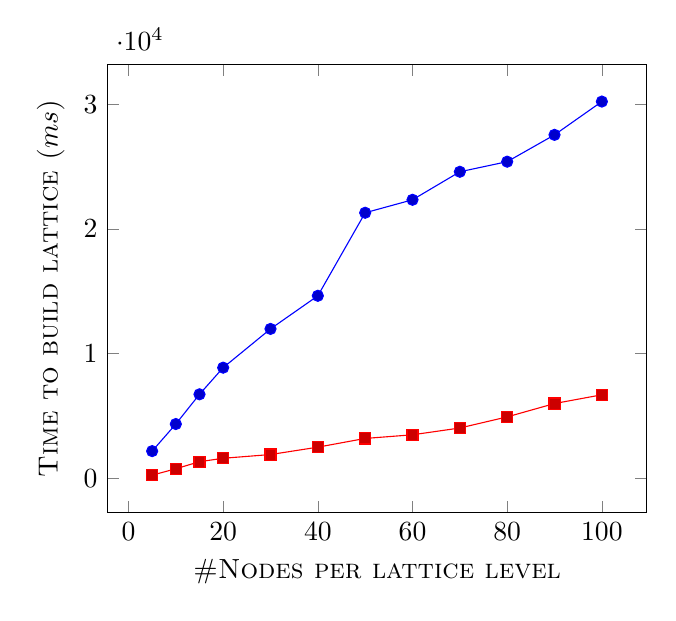
\begin{tikzpicture}[scale=1.0]
 \begin{axis}[
        xlabel=\textsc{\#Nodes per lattice level},
        ylabel=\textsc{Time to build lattice ($ms$)}
    ]
\addplot coordinates {(5,2165) (10,4337) (15,6723) (20,8860) (30,11969) (40,14626) (50,21288) (60,22329) (70,24577)
(80,25387) (90,27539) (100,30210)};
\addplot coordinates {(5, 235) (10,748) (15, 1317) (20, 1590) (30, 1890) (40, 2482) (50, 3182) (60, 3474) (70, 4020)
(80, 4911) (90,5982) (100,6684)};
\end{axis}
\end{tikzpicture}

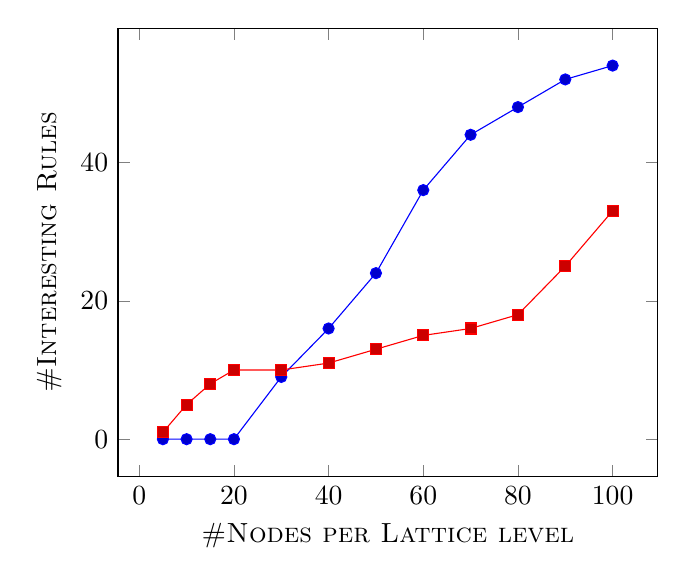
\begin{tikzpicture}[scale=1.0]
 \begin{axis}[
        xlabel=\textsc{\#Nodes per Lattice level},
        ylabel=\textsc{\#Interesting Rules}
    ]
\addplot coordinates {(5,0) (10,0) (15,0) (20, 0) (30, 9) (40,16) (50,24) (60,36) (70,44) (80,48) (90,52) (100,54)};
\addplot coordinates {(5,1) (10,5) (15,8) (20,10) (30,10) (40,11) (50,13) (60,15) (70,16) (80,18) (90,25) (100,33)};
\end{axis}
\end{tikzpicture}
\end{figure}

\begin{figure}
 \caption{Lattice with 4 levels}
 \centering
 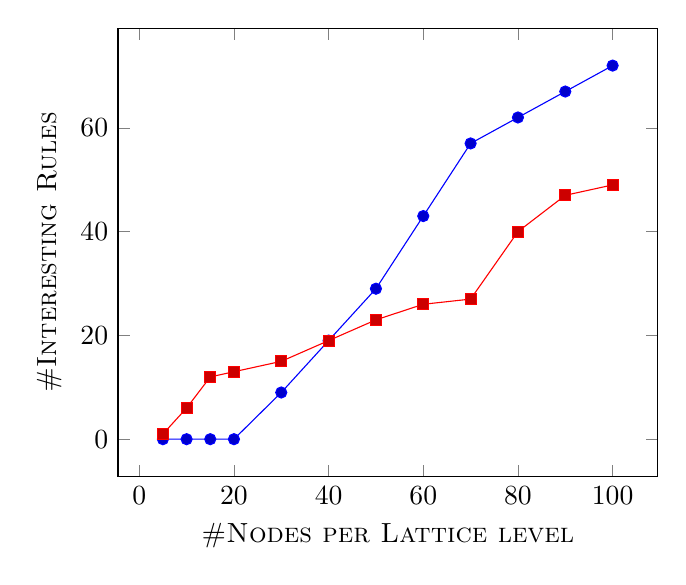
\begin{tikzpicture}[scale=1.0]
  \begin{axis}[
	  xlabel=\textsc{\#Nodes per Lattice level},
	  ylabel=\textsc{\#Interesting Rules}
      ]
  \addplot coordinates {(5,0) (10,0) (15, 0) (20, 0) (30, 9) (40,19) (50,29) (60,43) (70,57) (80,62) (90,67) (100,72)};
  %(110,75) (120,79) (130,84) (140,88) (150,94) (200,122) (250,159) (300,178) (350,200) (400,214) (450,231) (500,242)};
  \addplot coordinates {(5,1) (10,6) (15,12) (20,13) (30,15) (40,19) (50,23) (60,26) (70,27) (80,40) (90,47) (100,49)};
  %(110,) (120,) (130,) (140,) (150,) (200,) (250,) (300,) (350,) (400,) (450,) (500,)};
  \end{axis}
  \end{tikzpicture}
  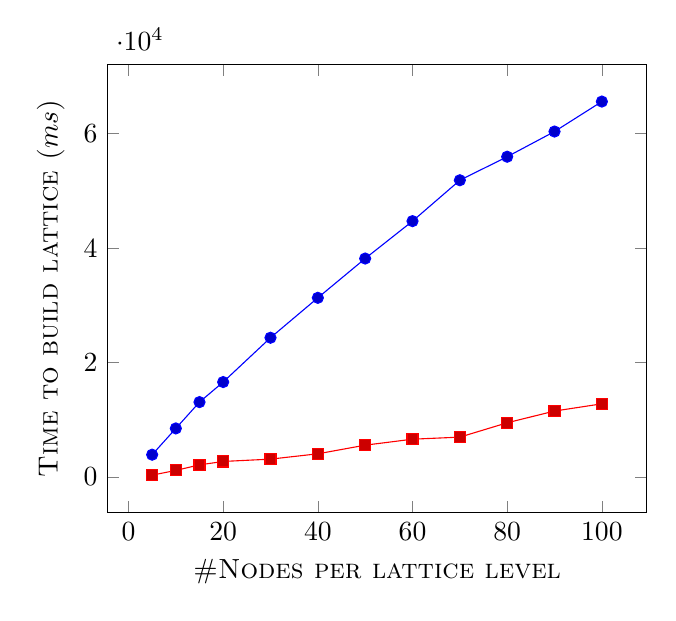
\begin{tikzpicture}[scale=1.0]
  \begin{axis}[
	  xlabel=\textsc{\#Nodes per lattice level},
	  ylabel=\textsc{Time to build lattice ($ms$)}
      ]
  \addplot coordinates {(5,3905) (10,8496) (15,13097) (20,16601) (30,24348) (40,31322) (50,38189) (60,44724) (70,51869)
  (80,55981) (90,60382) (100,65622)};
% (110,75) (120,79) (130,84) (140,88) (150,94) (200,122) (250,159) (300,178)  (350,200) (400,214) (450,231) (500,242)};
  \addplot coordinates {(5, 330) (10,1161) (15, 2128) (20, 2722) (30, 3130) (40, 4060) (50, 5571) (60, 6613) (70, 6976)
  (80, 9483) (90,11534) (100,12795)};
% (110,) (120,) (130,) (140,) (150,) (200,) (250,) (300,) (350,) (400,) (450,) (500,)};
  \end{axis}
  \end{tikzpicture}
\end{figure}

\begin{figure}
 \caption{Recall-Accuracy }
 \centering
 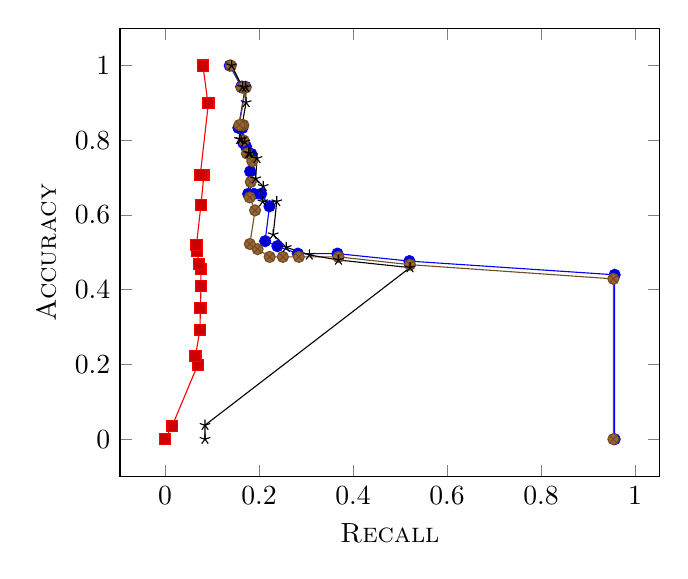
\begin{tikzpicture}[scale=1.0]
  \begin{axis}[
	  xlabel=\textsc{Recall},
	  ylabel=\textsc{Accuracy}
      ]
  \addplot coordinates {(0.9565217,0) (0.9565217,0.44) (0.52,0.4766667) (0.3669951,0.4966667) (0.2827325 ,
0.4966667) (0.2391975,0.5166667) (0.2131367,0.53) (0.2223543,0.6233333) (0.2045691,0.6566667) (0.1894231 ,
0.6566667) (0.1769991,0.6566667) (0.1812816,0.7166666) (0.1839358,0.7633333) (0.1724138,0.7833334) (0.1665500 ,
0.7933334) (0.1649076,0.8333333) (0.1612903,0.8333333) (0.15625,0.8333333) (0.1711004,0.9433333) (0.1644393 ,
0.9433333) (0.1623637,0.9433333) (0.1379310,1)};
  \addplot coordinates {(0,0) (0,0) (0,0) (0,0) (0.01530612,0.03508772) (0.0698152,0.1988304) (0.06495727 ,
0.2222222) (0.07440476,0.2923977) (0.07556675,0.3508772) (0.07667032,0.4093567) (0.07617188,0.4561403)
(0.07181329,0.4678363) (0.06907631,0.502924) (0.06711916,0.5204678) (0.0764832,0.625731) (0.0829904,0.7076023)
(0.0810992,0.7076023) (0.07846952,0.7076023) (0.07520199,0.7076023) (0.09260373,0.9005848) (0.09139466 ,
0.9005848) (0.08077468,1)};
  \addplot coordinates { (0.9538462,0) (0.9538462,0.4290657) (0.5212355,0.467128) (0.3691100,0.4878893)
(0.2848485,0.4878893) (0.2508897,0.4878893) (0.2227488,0.4878893) (0.1970509,0.5086505) (0.180622,0.5224913)
(0.1917660,0.6124567) (0.1803279,0.6470588) (0.1825688,0.6885813) (0.1858254,0.7439446) (0.1744278,0.7647059)
(0.1676343,0.799308) (0.1667810,0.8408305) (0.1631968,0.8408305) (0.1583062,0.8408305) (0.1718256,0.9411765)
(0.1654501,0.9411765) (0.1634615,0.9411765) (0.1401552,1)};
  \addplot coordinates {(0.08527132,0) (0.08527132,0.03741496) (0.5212355,0.4591837) (0.3691100,0.4795918)
(0.3072034,0.4931973)
(0.2581197,0.5136054) (0.2303290,0.547619) (0.2379135,0.6360544) (0.2080089,0.6360544) (0.2090336,0.6768708)
(0.193032,0.6972789) (0.1957484,0.7517007) (0.1810137,0.7653061) (0.1781473,0.7653061) (0.1696882,0.7959183)
(0.1621993,0.8027211) (0.1587088,0.8027211) (0.1726384,0.9013606) (0.1716233,0.9421769) (0.1653731,0.9421769)
(0.1418234,1)};
  \end{axis}
  \end{tikzpicture}
\end{figure}

\begin{figure}
 \caption{Runtime-LearnedRules}
 \centering
 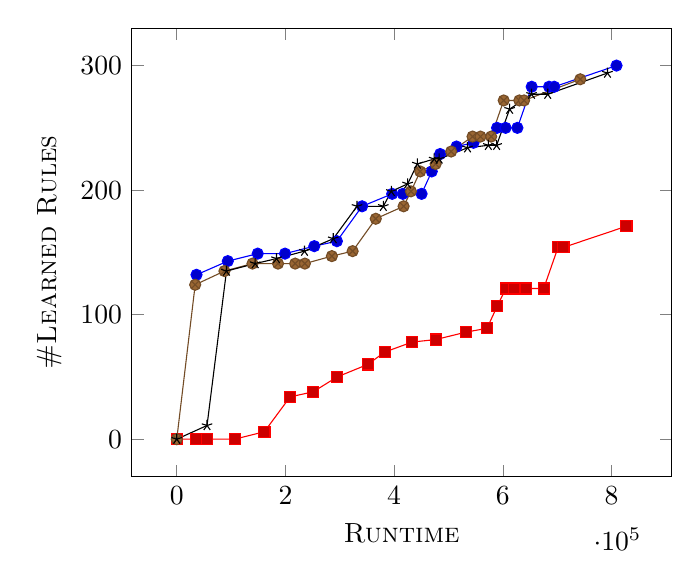
\begin{tikzpicture}[scale=1.0]
  \begin{axis}[
	  xlabel=\textsc{Runtime},
	  ylabel=\textsc{\#Learned Rules}
      ]
  \addplot coordinates { (36343,132) (93944,143) (148944,149) (199223,149) (253104,155) (294678,159) (341024,187)
(396459,197) (416000,197) (450504,197) (469231,215) (484591,229) (514785,235) (546069,238) (589417,250) (605128,250)
(626821,250) (653140,283) (685085,283) (694687,283) (809238,300)};
  \addplot coordinates {(0,0) (35466,0) (55421,0) (106586,0) (161302,6) (208629,34) (250863,38) (295212,50) (351300,60)
(382899,70) (433423,78) (476677,80) (532442,86) (570818,89) (589925,107) (605518,121) (621333,121) (643190,121)
(675208,121) (701631,154) (711515,154) (827520,171)};
  \addplot coordinates {(0,0) (33892,124) (87747,135) (139353,141) (186294,141) (217893,141) (235750,141) (285443,147)
(323626,151) (366197,177) (417438,187) (430932,199) (447970,215) (476371,221) (504948,231) (544307,243) (558897,243)
(578569,243) (601647,272) (630384,272) (639120,272) (742514,289)};
  \addplot coordinates {(0,0) (55709,11) (91488,135) (144319,141) (183567,145) (235053,151) (288040,161) (331747,187)
(380080,187) (394814,199)
(424827,205) (442860,221) (473691,225) (482918,225) (535099,234) (573386,236) (588600,236) (612505,265) (652833,277)
(682636,277) (792557,294)};
  \end{axis}
  \end{tikzpicture}
\end{figure}


\subsection{Example of Rules Learned}

We selected a couple of interesting rules learned with our approach in order to illustrate the kind of results we
obtain. On LinkedMDB, for example, we learned that films in English with Canadian director, and low budget are
significantly more likely to be also Canadian than the ones with higher budget. The base rule shown below has
confidence $0.36$:

$country(X,canada)$ :- $director(X,Z),bornIn(Z,canada),language(X,english),budget(X,Y)$

When we refine this rule, we find an interval with confidence $0.83$:

$country(X,canada)$ :- $director(X,Z),bornIn(Z,canada),language(X,english),budget(X,Y),Y\leq 80000$

